 \chapter{Arquitetura}
\label{sec:arquitetura}

A arquitectura é uma etapa fundamental em todos os projecto porque é aqui que se define a estrutura e comportamento do sistema na sua globalidade e nas diferentes componentes.

Neste capítulo está exposta a arquitectura do 10.quest que servirá de \textit{guideline} para a implementação do projecto. Serão apresentadas diferentes prespectivas para analisar os diferentes aspectos do sistema. É de notar que as componentes a desenvolver pela restante equipa de desenvolvimento não será analisada e apenas será apresentada de forma superficial para fazer a ligação às componentes a desenvolver no ambito do estágio curricular.
Este capítulo é também uma exposição das decisões arquitecturais efectuadas no primeiro semestre, respeitando as restrições técnicas e de negócios.

Por fim será feita uma analise dos riscos envolvidos no desenvolvimento do projecto, o seu impacto e probabilidade de ocurrência e o respectivo plano de mitigação




\section{Analise da Arquitectura}
\label{analisearq}

Na analise da arquitectura serão apresentadas as restrições do projecto, que têm um impacto directo nas decisões de arquitectura, as diferentes prespectivas de arquitetura e as técnologias utilizadas.

\subsection{Restrições Técnicas}
As restrições técnicas são decisões técnicas arquiteturais que devem ser satisfeitas. O Sistema a desenvolver deve respeitar as seguintes restrições:

\textbf{Identificador: RT01}
\newline
\textbf{Título:} Arquitectura REST
\newline
\textbf{Descrição:} A comunicação entre a plataforma a desenvolver e o TCG deve seguir uma arquitectura REST.

\textbf{Identificador: RT02}
\newline
\textbf{Título:} Base de Dados
\newline
\textbf{Descrição:} Os dados utilizados pela aplicação devem ser guardados numa base de dados, visto tratar-se de um grande volume de dados que tem de permanecer organizado. Relativamente aos dados do TCG foi imposto que os dados não sejam duplicados e que esta informação seja acedida através de pedidos HTTP/REST. PostegreSQL\cite{sql} é a base de dados relacional utilizada pela empresa e portanto será também utilizada no desenvolvimento deste projecto.

\textbf{Identificador: RT03}
\newline
\textbf{Título:} Framework Django\cite{django}
\newline
\textbf{Descrição:} A Framework Django é a técnologia utilizada pela empresa para desenvolver aplicações \textit{web} e \textit{\acrshort{saas}}. O uso desta técnologia foi imposta pelo \textit{Product Owner}.

\textbf{Identificador: RT04}
\newline
\textbf{Título:} Plataforma Web
\newline
\textbf{Descrição:} Todas as funcionalidades do sistema devem estar disponíveis através da plataforma web.

\subsection{Restrições de Negócio}
Nesta secção estão descritas as restrições de negócio, que podem ser entendidas com barreiras que a organização deve lutar para executar a sua estratégia. Estas restrições seguintes foram impostas pelo \textit{Product Owner} e devem ser satisfeitas na arquitectura do sistema:

\textbf{Identificador: RN01}
\newline
\textbf{Título:} Programa de Desenvolvimento
\newline
\textbf{Descrição:} O produto deve estar concluido e validado até dia 15 de Junho.



\subsection{\acrfull{mvc}}

A estrutura de um projeto Django é muitas vezes descrito como um projeto \acrshort{mvc}. Como podemos ver na Figura \ref{fig:arq-mvc}, o modelo \acrshort{mvc} é uma arquitectura de sowftare que separa a aplicação em três componentes lógicos principais. Por outras palavras este modelo separa a apresentação dos dados, da lógica que trata das \textit{interfaces} do utilizador, facilitando a programação das diferentes funcionalidades, \textit{debugging} e os testes das mesmas.

\begin{figure}[ht!]
	\begin{center}
		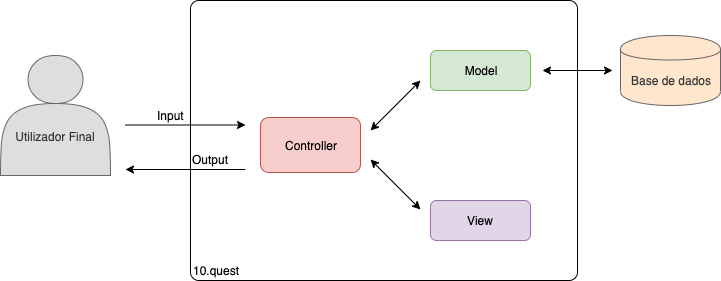
\includegraphics[width=1\textwidth]{img/arq/diagrama-MVC}
		\caption{Estrutura do Sistema}
		\label{fig:arq-mvc}
	\end{center}
\end{figure}

O componente \textbf{Model} controla a organização e armazenamento dos dados. Este módulo representa os dados que são transferidos entre os componentes Controller e View mas não representa nenhuma lógica no que diz respeito ao que é representado na camada de apresentação.

O componente \textbf{View} pode ser considerada a camada de apresentação. Este componente contém todas os ingredientes que constituem as interfaces do utilizador e controla a forma como a informação lhe é apresentada. Este modelo sabe como aceder ao modelo de dados que é apresentado ao utilizador contudo não sabe como o manipular nem o que significa.

Por último temos o componente \textbf{Controller}.  Este componente atua entre os modelos View e Model reagindo a eventos na View e respondendo a estes pedidos manipulando os dados utilizando o componente Model e interagindo com o componente View para renderizar o \textit{output}.


\subsection{Modelo C4}

Nesta secção encontra-se representada e descrita toda a arquitetura da plataforma 10.quest,  influênciada pelos objetivos de negócio, \textit{stakeholders}, requisitos e restrições técnica e de negócio, apresentados anteriormente.

Foram utilizados três diagramas para representar a arquitectura do sistema, utilizando o \textbf{modelo C4}\cite{c4}: diagrama de contexto, diagrama de contentores, diagrama de componentes e o diagrama de classes.

Os diferentes diagramas representam diferentes perspectivas e níveis de abstração e foram feitos com o intuito de facilitar a compreensão da arquitetura permitindo à equipa de desenvolvimento visualizar os diferentes níveis de granularidade. 

O diagrama de contexto mostra a relação entre o sistema que vai ser desenvolvido e outros agentes como por exemplo utilizadores e sistemas externos.  Este é o diagrama com maior nível de abstração e é bom para sublinhar as dependencias externas que a equipa de desenvolvimento tem que integrar no sistema. 

O diagrama de contentores apresenta um maior detalhe (i. e. relativamente ao diagrama de contexto) e motras os diferentes contentores que constituem o sistema (e. g. bases de dados, aplicações, microserviços etc...). Neste diagrama são também definidas algumas decisões arquitecturais. 

Por último temo o diagrama de componentes aproxima um contentor individualmente e mostra todos os componentes que constituem esse contentor. Desta forma conseguimos perceber as principais funcionalidades do sistema. 

\begin{figure}[ht!]
	\begin{center}
		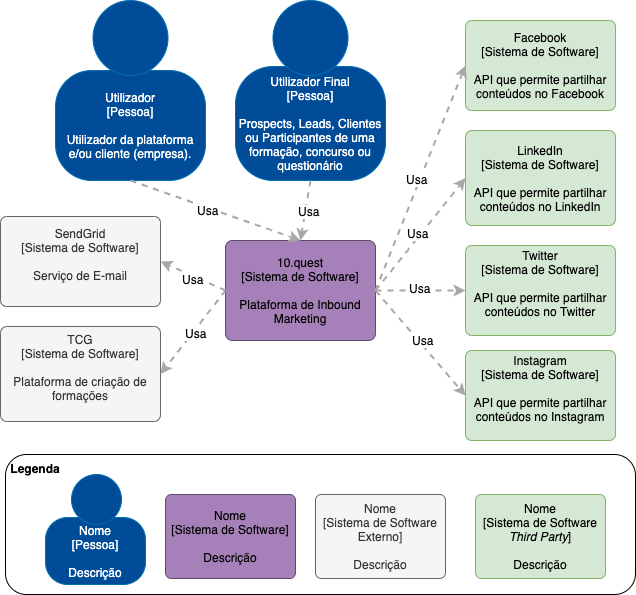
\includegraphics[width=1\textwidth]{img/arq/diagrama-contexto}
		\caption{Diagrama de Contexto}
		\label{fig:arq-contexto}
	\end{center}
\end{figure}

\begin{figure}[ht!]
	\begin{center}
		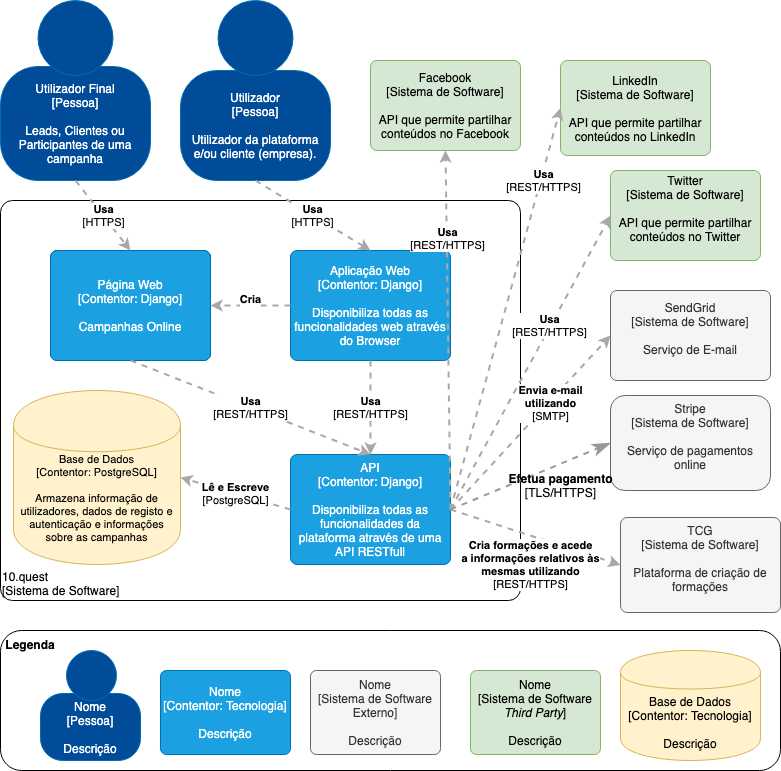
\includegraphics[width=1\textwidth]{img/arq/diagrama-contentores}
		\caption{Diagrama de Contentores}
		\label{fig:arq-contentores}
	\end{center}
\end{figure}

\begin{figure}[ht!]
	\begin{center}
		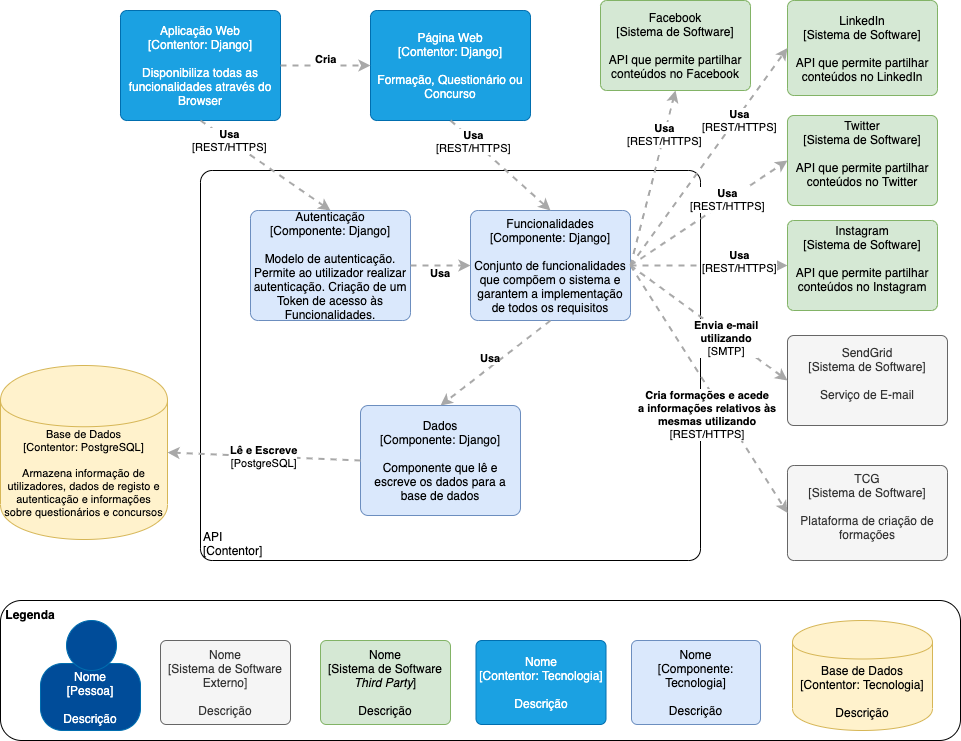
\includegraphics[width=1\textwidth]{img/arq/diagrama-componentes}
		\caption{Diagrama de Componentes}
		\label{fig:arq-componentes}
	\end{center}
\end{figure}

\begin{figure}[ht!]
	\begin{center}
		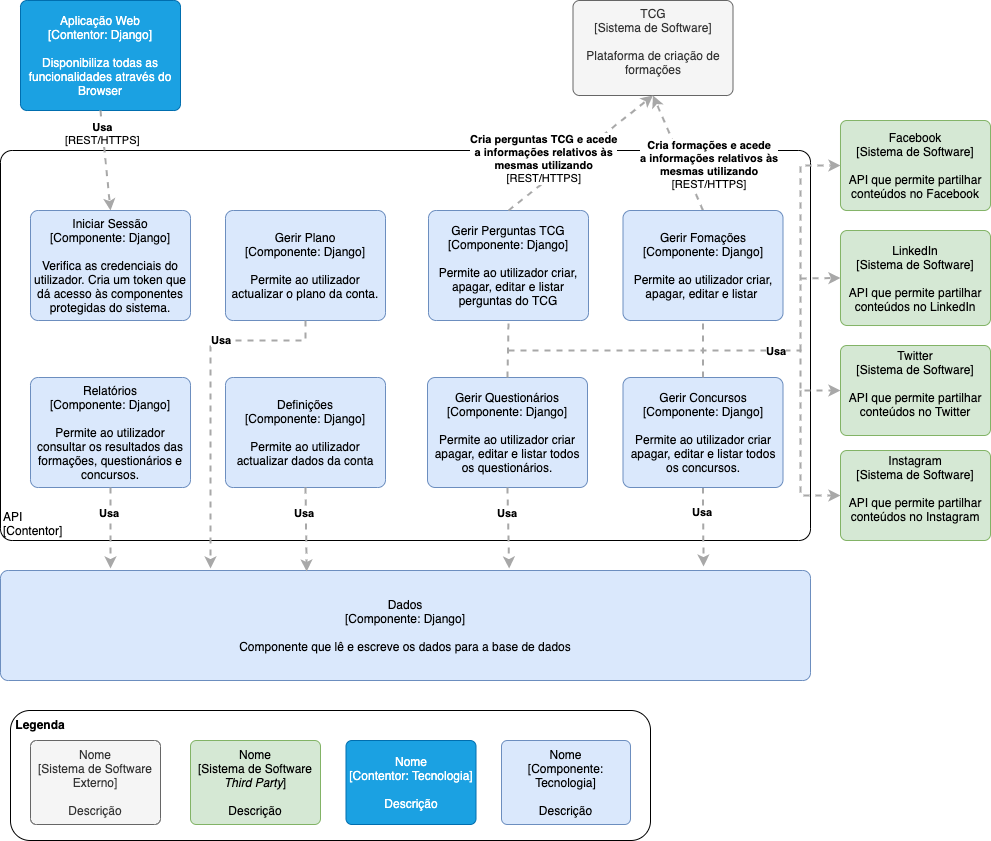
\includegraphics[width=1\textwidth]{img/arq/diagrama-componentes1}
		\caption{Diagrama Componentes da componente Funcionalidades}
		\label{fig:arq-componentes1}
	\end{center}
\end{figure}

\subsection{Modelo Sequencial}

\subsection{Modelo de Dados}

\subsection{Técnologias Utilizadas}

\section{Analise de Riscos}
\label{analiseriscos}
%-------------------------------------------------------------------------------------------------
\blankpage
%-------------------------------------------------------------------------------------------------

\glsresetall
